\documentclass{report}
% Include all project wide packages here.
\usepackage{fullpage}
\usepackage[style=ieee]{biblatex}
\usepackage[dutch]{babel}

\renewcommand{\familydefault}{\sfdefault}

\setmainfont[Ligatures=TeX]{Myriad Pro}
\setmathfont{Asana Math}
\setmonofont{Lucida Console}

\usepackage{titlesec, blindtext, color}
\definecolor{gray75}{gray}{0.75}
\newcommand{\hsp}{\hspace{20pt}}
\titleformat{\chapter}[hang]{\Huge\bfseries}{\thechapter\hsp\textcolor{gray75}{|}\hsp}{0pt}{\Huge\bfseries}
\renewcommand{\familydefault}{\sfdefault}
\renewcommand{\arraystretch}{1.2}
\setlength\parindent{0pt}

%For code listings
\definecolor{black}{rgb}{0,0,0}
\definecolor{browntags}{rgb}{0.65,0.1,0.1}
\definecolor{bluestrings}{rgb}{0,0,1}
\definecolor{graycomments}{rgb}{0.4,0.4,0.4}
\definecolor{redkeywords}{rgb}{1,0,0}
\definecolor{bluekeywords}{rgb}{0.13,0.13,0.8}
\definecolor{greencomments}{rgb}{0,0.5,0}
\definecolor{redstrings}{rgb}{0.9,0,0}
\definecolor{purpleidentifiers}{rgb}{0.01,0,0.01}


\lstdefinestyle{csharp}{
language=[Sharp]C,
showspaces=false,
showtabs=false,
breaklines=true,
showstringspaces=false,
breakatwhitespace=true,
escapeinside={(*@}{@*)},
columns=fullflexible,
commentstyle=\color{greencomments},
keywordstyle=\color{bluekeywords}\bfseries,
stringstyle=\color{redstrings},
identifierstyle=\color{purpleidentifiers},
basicstyle=\ttfamily\small}

\lstdefinestyle{c}{
language=C,
showspaces=false,
showtabs=false,
breaklines=true,
showstringspaces=false,
breakatwhitespace=true,
escapeinside={(*@}{@*)},
columns=fullflexible,
commentstyle=\color{greencomments},
keywordstyle=\color{bluekeywords}\bfseries,
stringstyle=\color{bluestrings},
identifierstyle=\color{purpleidentifiers}
}

\lstdefinestyle{vhdl}{
language=VHDL,
showspaces=false,
showtabs=false,
breaklines=true,
showstringspaces=false,
breakatwhitespace=true,
escapeinside={(*@}{@*)},
columns=fullflexible,
commentstyle=\color{greencomments},
keywordstyle=\color{bluekeywords}\bfseries,
stringstyle=\color{redstrings},
identifierstyle=\color{purpleidentifiers}
}

\lstdefinestyle{xaml}{
language=XML,
showspaces=false,
showtabs=false,
breaklines=true,
showstringspaces=false,
breakatwhitespace=true,
escapeinside={(*@}{@*)},
columns=fullflexible,
commentstyle=\color{greencomments},
keywordstyle=\color{redkeywords},
stringstyle=\color{bluestrings},
tagstyle=\color{browntags},
morestring=[b]",
  morecomment=[s]{<?}{?>},
  morekeywords={xmlns,version,typex:AsyncRecords,x:Arguments,x:Boolean,x:Byte,x:Char,x:Class,x:ClassAttributes,x:ClassModifier,x:Code,x:ConnectionId,x:Decimal,x:Double,x:FactoryMethod,x:FieldModifier,x:Int16,x:Int32,x:Int64,x:Key,x:Members,x:Name,x:Object,x:Property,x:Shared,x:Single,x:String,x:Subclass,x:SynchronousMode,x:TimeSpan,x:TypeArguments,x:Uid,x:Uri,x:XData,Grid.Column,Grid.ColumnSpan,Click,ClipToBounds,Content,DropDownOpened,FontSize,Foreground,Header,Height,HorizontalAlignment,HorizontalContentAlignment,IsCancel,IsDefault,IsEnabled,IsSelected,Margin,MinHeight,MinWidth,Padding,SnapsToDevicePixels,Target,TextWrapping,Title,VerticalAlignment,VerticalContentAlignment,Width,WindowStartupLocation,Binding,Mode,OneWay,xmlns:x}
}

%defaults
\lstset{
basicstyle=\ttfamily\small,
extendedchars=false,
numbers=left,
numberstyle=\ttfamily\tiny,
stepnumber=1,
tabsize=4,
numbersep=5pt
}
\addbibresource{../../library/bibliography.bib}

\title{EPO-2: Mid-term Design Report - 7-segment display}
\author{Joris Blom}

\begin{document}

\chapter{7-segmentendisplay}
\label{ch:sseg}
\section{Eisen}
\label{sec:Eisen}
Het 7-segmentendisplay moet aan de volgende eisen voldoen: 
\begin{itemize}
\item Het 7-segmentendisplay moet door middel van een 16 bits input de hexadecimale cijfers 0 t/m F op elk 7-segmenten-display kunnen weergeven
\item Het 7-segmentendisplay moet door middel van een 4 bits input de punten van elk 7-segment display los kunnen aansturen
\item Het 7-segmentendisplay moet de state van de zender, ontvanger en het main-FSM kunnen weergeven
\end{itemize}

\section{Implementatie}
De 7-segmentendisplays worden gebruikt om de verschillende states van de ontvanger, zender en het main-FSM weer te geven.
Het meest linkse 7-segmentendisplay wordt niet gebruikt.
Het 7-segmentendisplay rechts van het midden wordt gebruikt om de state van de zender te weergeven.
Het display links van het midden wordt gebruikt om de state van de ontvanger te weergeven, en het meest linkse display wordt gebruikt om de state van de main-FSM te weergeven.
De punten onder de displays hebben geen functie en staan altijd uit.

\begin{figure}[H]
\centering
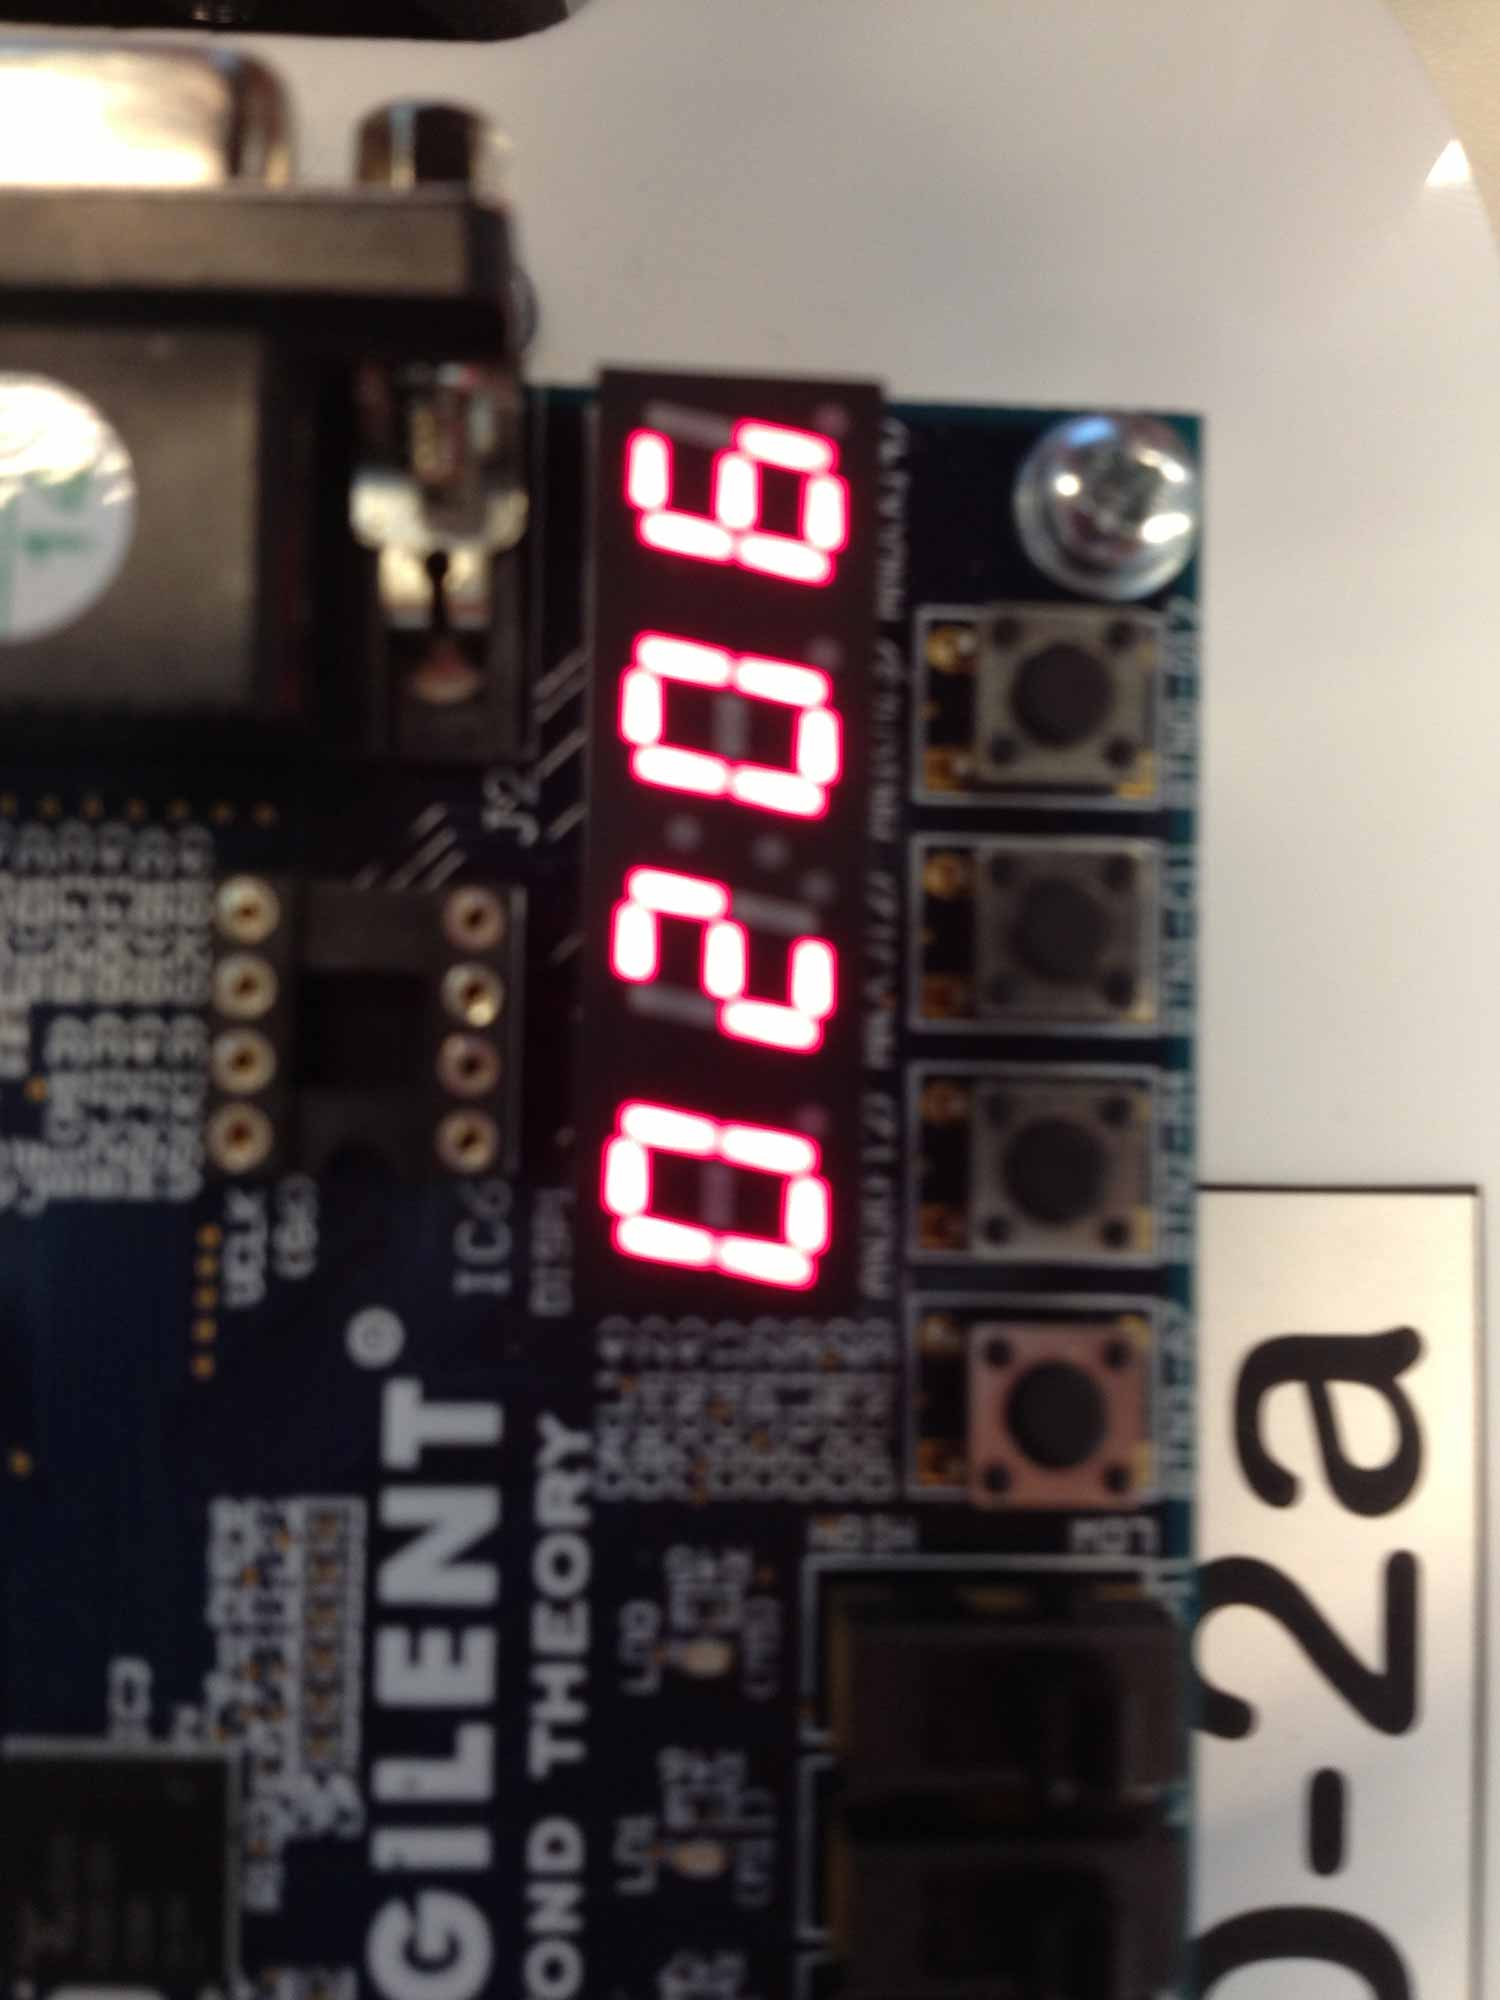
\includegraphics[width=0.6\textwidth]{7_segment_display-robot.jpg}

\caption{7-segmentendisplay-robot}
\end{figure}

\newpage
\section{Werkingsprincipe}
De controller stuurt een 16 bits vector en een 4 bits vector naar de displayaansturing.
Het display wordt aangestuurd door de FPGA, die door middel van VHDL geprogrammeerd is.
De 16 bits vector stuurt de 7 segmenten aan en de 4 bits vector de punt onder het 7-segmentendisplay.
In de VHDL-code wordt de 16 bit vector opgedeeld in 4 bits-vectoren.
Elk van deze 4 bits-vectoren wordt weergegeven op 1 van de displays als hexadecimale waarde.
\begin{figure}[H]
\centering
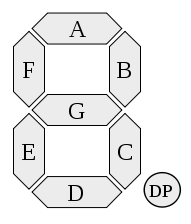
\includegraphics[width=0.3\textwidth]{7_segment_display.png}

\caption{7-segmentendisplay}
\end{figure}
Hierboven is een afbeelding te zien van \'{e}\'{e}n 7-segment display.
Elke letter correspondeerd met een led om de verschillende leds te kunnen onderscheiden.
Hieronder is het complete schema te zien van de vier 7-segment displays, hier worden de zelfde letters gebruikt.

Alle leds per 7-segmentendisplay hebben een gezamenlijke voedingsspanning, dus alle 8 anodes per display zijn elektrisch verbonden (zie figuur \ref{fig:ssegschematic}).
Hierdoor kan elk 7-segmentendisplay afzonderlijk aan en uit worden geschakeld.
Door middel van de kathodes kunnen de leds afzonderlijk aan en uit worden gezet.
De kathodes van de leds met dezelfde letter zijn elektrische met elkaar verbonden (zie figuur \ref{fig:ssegschematic}).
Er kan dus maar 1 letter of cijfer tegelijk op alle 4 de displays worden weergeven.
Door de displays door middel van de anode om de beurt afzonderlijk aan en uit te zetten op een hoge frequentie kunnen alle 4 de displays apart aangestuurd worden.
Door de hoge frequentie is het voor het menselijk oog niet te zien dat het display knippert.
\begin{figure}[H]
\centering

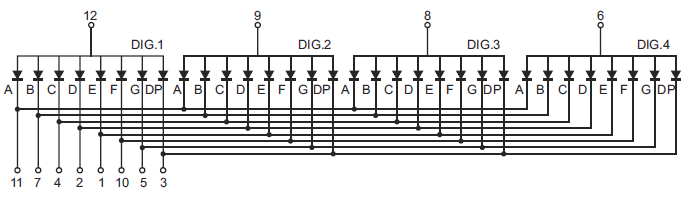
\includegraphics[width=0.7\textwidth]{7_segment_display_schematic.png}

\caption{7-segmentendislplay schematic}
\label{fig:ssegschematic}
\end{figure}


\end{document}